\section{Diferenciación}

\begin{defn}[Función\IS diferenciable]
 $F$ es diferenciable en $\gor{a}$ si existe una aplicación lineal $L$ tal que
 
\[ \frac{F(\gx)-F(\ga)-L(\gx-\ga)}{||\gx-\ga||} \convs[][\gx][\ga] 0 \]

que se puede expresar como
\[ \lim_{\gor{h} \rightarrow \gor{0}} \frac{\md{F(\ga+\gor{h}) - F(\ga) - L\gor{h}}}{||\gor{h}||} = 0 \]
\end{defn}

\begin{defn}[Diferencial]
A esa matrix $L$ la vamos a llamar la diferencial de $F$ en $\ga$:

\[ L\equiv DF(\ga) \]
\end{defn}

\begin{theorem} 
$$F \text{ diferenciable en } \ga \implies F \text{ continua en } \ga$$
\end{theorem}

\begin{proof}
 $$\lim_{\gor{h} \rightarrow \gor{0}} \frac{\md{F(\ga+\gor{h}) - F(\ga) - L\gor{h}}}{\md{\gor{h}}} = 0$$
 Esta es la definición de diferenciable. Para que este límite sea 0, el numerador tiene que tender a 0, por lo que $F(\ga+\gor{h}) - F(\ga) \rightarrow 0$
\end{proof}


\begin{theorem} 
Si la diferencial existe, entonces es única.
\end{theorem}

\begin{proof}  Vamos a demostrar que esa aplicación $L$ es única. Supongamos que existen $L_1,L_2$ que cumplen las condiciones.
\[0=\lim_{\gor{h} \rightarrow \gor{0}} \frac{F(\gor{a}+\gor{h}) - F(\ga)-L_1\gor{h}}{||\gor{h}||} = \lim_{\gor{h} \rightarrow \gor{0}} \frac{F(\gor{a}+\gor{h}) - F(\ga)-L_2\gor{h}}{||\gor{h}||}\].

Sumando:

\[ 0 = \lim_{\gor{h} \rightarrow \gor{0}} \frac{||F(\gor{a}+\gor{h}) - F(\ga)-L_1\gor{h}|| + ||F(\gor{a}+\gor{h}) - F(\ga) -L_2\gor{h}||}{||\gor{h}||} \]

Teniendo en cuenta que $||A-B|| = ||A+(-B)|| \leq ||A||+||B||$

\[ 0 \leq \lim_{\gor{h} \rightarrow \gor{0}} \frac{2\cdot\md{F(\ga + \gor{h}) - F(\ga)} + \md{L_1\gor{h}} + \md{L_2\gor{h}}}{\md{\gor{h}}} \]

\textit{Aquí falta completar.}
\end{proof}



\paragraph{Nomenclatura: }
Aproximación lineal $\sim$ Diferencial.

Matriz jacobiana $\sim$ Jacobiana.

\begin{defn}[Matriz\IS diferencial]
 Matriz asociada a $DF(\ga) \equiv $ Matriz de las derivadas parciales de F.
 
 $$DF(\ga) \equiv \begin{pmatrix}
                \dpa{F_1}{x_1} & \cdot & \dpa{F_1}{x_N}\\
                \vdots& \ddots & \vdots\\
                \dpa{F_N}{x_1} & \cdot & \dpa{F_N}{x_N}
                \end{pmatrix}
$$
\end{defn}

\begin{theorem}
 $F$ diferenciable en $\ga \implies \exists \deriv{F_k}{x_i}(\ga), i=1,2,...,N \y k = 1,2,...,M$
\end{theorem}

El contraejemplo para demostrar la implicación a la izquierda es el mismo que en los límites a lo largo de rectas.

$f(x,y) = \left\{ \begin{matrix}

\frac{xy^2}{x+y^2} & (x,y) = (0,0) \\ 
0 & (x,y)=(0,0)
           
          \end{matrix}\right.
$

Según las aplicaciones que tengamos, la diferencial se suele llamar de una u otra forma. Con $\appl{\delta}{\real}{\real^M}$ utilizamos notación vectorial en vez de matricial porque tendríamos una matriz columna. Por ejemplo: la velocidad (en un instante de tiempo, un punto en el espacio).

\begin{defn}[Gradiente] Sea $\appl{F}{\real^N}{\real}$, entonces definimos el vector gradiente como 

\[ \grad F(\gx) = DF(\gx) = \left(\dpa{F}{x_1}, \dpa{F}{x_2},\dotsc, \dpa{F}{x_n}\right) \]
\end{defn}


\subsection{Regla de la cadena}
\index{Regla!de la cadena}
Consideremos la composición de dos funciones de la siguiente forma:

$\appl{F}{\real^N}{\real^M}$. 

$\appl{G}{\real^M}{\real^K}$.

$\appl{H=G\circ F}{\real^N}{\real^K}$.

$ \gx \in \real^N, \gy \in \real^M$

\begin{wrapfigure}{r}{0.3\textwidth}
\begin{center}
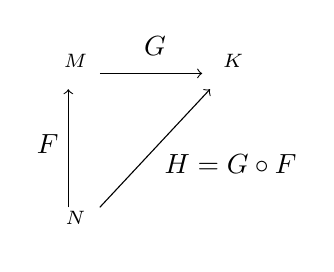
\begin{tikzpicture}
\draw[->] (-0.1,0.2) -- (-0.1,1.7);
\draw[->] (0.3,1.9) -- (1.6,1.9);
\draw[->] (0.3,0.2) -- (1.7,1.7);

\node at (0,0) {$\real^N$};
\node at (0,2) {$\real^M$};
\node at (2,2) {$\real^K$};

\node[left] at (-0.1,1) {$F$};
\node[above] at (1,2) {$G$};
\node[below right] at (1,1) {$H = G\circ F$};
\end{tikzpicture}
\end{center}
\caption{Composición de funciones}
\end{wrapfigure}

Con $F$ diferenciable en $\ga$ y $G$ diferenciable en $F(\gor{a})$. Entonces $H=G\circ F$ es diferenciable en $\ga $.
Además la expresión matricial es:

\[ \underbrace{DH(\ga)}_{K\times N} = \underbrace{DG(F(\ga))}_{K\times M}\cdot \underbrace{DF(\ga)}_{M\times N} \]
 
No hace falta calcular toda la matriz si sólo queremos un elemento. Para calcular 1 único elemento de la matriz diferencial (el de la fila $i$, columna $j$), usamos la siguiente fórmula
\[ \dpa{H_i}{x_j}(\ga) = \sum_{k=1}^M \dpa{G_i}{y_k}\cdot\dpa{F_k}{x_j} \]

Siempre teniendo en cuenta que $\displaystyle\dpa{G_i}{y_k}$ está evaluado en $F(\ga)$ y $\displaystyle\dpa{F_k}{x_j}$ está evaluado en $\ga$.

\subsection{Extensiones del teorema del Valor Medio}

El teorema anterior que vimos del valor medio era para funciones de una variable, y proponía lo siguiente:
\begin{theorem}[Teorema\IS del valor medio (una variable)]
\label{thmTVM1var}
Dada $\appl{f}{\real}{\real}$ diferenciable, se tiene que \[ f(b)-f(a) = f'(c)(b-a)\] para algún $c\in[a,b]$
\end{theorem}

Después el teorema lo extendimos a funciones de $\real^N$ en $\real$: dada $\appl{F}{\real^N}{\real}$ entonces definíamos
 
 \[ \sigma(t)  = t\gor{b}+(1-t)\gor{a} \] 
 
 y $g = F\circ \sigma$ era una aplicación de los reales a los reales, y entonces aplicando el teorema anterior teníamos que 
 
 \[ F(\gor{b}-\gor{a}) = g(1)-g(0)  = g'(s) \] 
 para algún $s\in[0,1]$.

Sin embargo, al tratar de extrapolar este resultado a una función $\appl{F}{\real^N}{\real^2}$ nos queda que 

 \[ F(\gor{b})-F(\ga) = \begin{pmatrix}
                         \pesc{\nabla F_1(\gor{c_1}),{\gor{b}-\ga}}\\
                         \pesc{\nabla F_2(\gor{c_2}),\gor{b}-\ga}
                        \end{pmatrix}
 \]
  Tenemos 2 $c$ distintos, uno para cada $f$, por lo que este teorema pierde sentido. Hay que buscar una extensión, otra formulación del teorema que nos permita aplicarlo a las funciones que estamos estudiando.
  
  \begin{theorem} [Teorema\IS del valor medio (varias variables)]
  \label{thmTVM}
  Sea $f \in C^1$ en un abierto que contenga $[a,b]$. Entonces 
  
  \[ \norm{F(\gor{b})-F(\ga)} \leq \md{DF(\gor{c})} \cdot \md{\gor{b}-\ga} \]
  
  Siendo $c$ un punto del segmento que une $\ga$ y $\gb$ en el que $\md{DF(tb+(1-t)a)}$ alcanza su máximo.
  \end{theorem}  
  
  \begin{proof}

Primero vamos a demostrar la siguiente desigualdad:

\begin{equation}
\label{eqnTVM1}
 \md{\int_0^1 F(t) \,dt}≤ \int_0^1 \md{F(t)}\,dt 
\end{equation}

Si tomamos \[ L = \int_0^1 F(t) \,dt \]  entonces

\[ \md{L}^2 = \md{\int_0^1 F(t) \,dt}^2 = \pesc{L,\int_0^1 F(t) \,dt} \]

Como $L$ es un vector constante, podemos meterlo en la integral y tenemos que 

\[ \pesc{L,\int_0^1 F(t) \,dt} = \int_0^1 \pesc{L, F(t)} ≤ \int_0^1 \md{L}\md{F(t)} = \md{L} \int_0^1 \md{F(t)} \]

y por lo tanto

\begin{gather*}
\md{L}^2 ≤ \md{L} \int_0^1 \md{F(t)} \\
\md{L} ≤ \int_0^1 \md{F(t)} \\
\md{\int_0^1 F(t) \,dt } ≤ \int_0^1 \md{F(t)}  
\end{gather*}

quedando así demostrada la desigualdad (\ref{eqnTVM1}).

Consideramos ahora 

\[ \md{F(\gb) - F(\ga)} \]

Si integramos $DF$ por el camino que va de $\ga$ a $\gb$ nos queda que 

\[ \md{F(\gb) - F(\ga)} = \md{\int_0^1 DF\left[\ga(1-t) + t\gb\right](\gb - \ga)\, dt } \]

que por (\ref{eqnTVM1}) 

\[ \md{F(\gb)-F(\ga)} ≤ \int_0^1 \md{DF\left[\ga(1-t) + t\gb\right](\gb - \ga)}\, dt  \leq  \int_0^1 \md{DF\left[\ga(1-t) + t\gb\right]}\md{\gb - \ga}\, dt \]

Nos fijamos en $\md{DF\left[\ga(1-t) + t\gb\right]}$. Al ser continua y estar definida en un conjunto compacto, entonces alcanza su máximo en algún punto $\gor{c}$ entre $\ga$ y $\gb$, por lo tanto

\[ \md{F(\gb) - F(\ga)} ≤  \int_0^1 \md{DF(\gor{c})}\md{(\gb - \ga)} = \md{DF(\gor{c})}\md{\gb - \ga} \]
  \end{proof}

Este teorema nos sirve, por ejemplo, para ver que si tenemos $\appl{F}{\real^N}{\real^M}, F \in C^1$, definida en un conjunto abierto y conexo y  $DF(\gx) \equiv 0\; \forall\gx$, entonces $F$ es constante.

\subsection{Derivada direccional}

$\appl{F}{\real^N}{\real^M}$ (escalar)

$\ga \sim$ Recta que pasa por $\ga$ con dirección $\gor{v}$.

$r(t) = \ga + t\gor{v}$. 

\obs
Como una recta tiene infinitos vectores directores (dependiendo de la longitud), siempre tomaremos vectores directores unitarios, con $\norm{\gor{v}} = 1$.


Vamos a estudiar: $g(t) = F(\ga + t\gor{v}) = F \circ r (t)$.

$t \sim 0 \dimplies \ga + t\gor{v} \sim \ga$
\begin{defn} [Regla de la cadena]
$$g'(0) = \displaystyle\lim_{h \rightarrow 0} \frac{g(h)-g(0)}{h} = \displaystyle\lim_{h \rightarrow 0} \frac{F(\ga+h\gor{v})-F(\ga)}{h} \equiv D_{\gor{v}}F(\ga)$$. 
\end{defn}

\obs
La existencia de $D_{\gor{v}}F(\ga), \forall \gor{v}\in \real^N$ NO garantiza que $F$ sea derivable.


Si sabemos que $F$ SÍ es diferenciable podemos usar la regla de la cadena obteniendo:

$D_{\gor{v}}F(\ga) = g'(0) = D(F\circ r)(0) = ... = \pesc{\nabla F(\ga),\gor{v}}$


\paragraph{Aplicación:} 
\begin{itemize}
 \item 
 Dirección de máximo crecimiento:

$D_{\gor{v}}F(\ga) = \pesc{\nabla F(\ga),\gor{v}}\leq \norm{\nabla F(\ga)}\cdot \underbrace{\norm{\gor{v}}}_{\equiv 1}$

Conclusión:
\begin{align*}
D_{\gor{v}}F(\ga) &\leq \norm{\nabla F(\ga)}\\
&\uparrow\\
\text{El }= \text{se obtien}&\text{e cuando }\gor{v} = \displaystyle \frac{\nabla F(\ga)}{\norm{\nabla F(\ga)}}. 
\end{align*}

 
 \item
 Vector perpendicular a los conjuntos de nivel
 
 $\appl{F}{\real^N}{\real^M}$
 
 $S = \{ \gx \in \real^N \tq F(\gx) = 0\}$ (Conjunto de nivel)
 
 $\ga \in S$
 
 Entonces: $\nabla F(\ga) \perp S$
\end{itemize}

\begin{theorem}[Derivadas parciales continuas implican función diferenciable]
Si existen todas las derivadas parciales y son continuas $\implies F$ diferenciable en $\ga$.
 
\end{theorem}

Contraejemplo de la no reciprocidad: $f(x) = x^2 sin\left(\frac{1}{x}\right)$

\begin{proof}
 $\appl{F}{\real^2}{\real}$
 
 $$¿\frac{\left|F(a+a,b+k) - F(a,b) - \deriv{F}{x}(a,b) h - \deriv{F}{y}(a,b)k\right|}{\norm{(h,k)}}\longrightarrow 0?$$
 
 Sumamos y restamos al numerador $F(a,b+k)$.
 
 $$\frac{\left|\left(\underbrace{F(a+h,b+k) - F(a,b+k)}_{\deriv{F}{x}(a+\tilde{h},b+k) \text{ para algún } 0 \leq\tilde{h}\leq h} -  \deriv{F}{x}(a,b) h\right) + \left(\underbrace{F(a,b+k) - F(a,b)}_{\deriv{F}{x}(a+h,b+\tilde{k}) \text{ si } 0 \leq\tilde{k}\leq k}- \deriv{F}{y}(a,b) k\right)\right|}{\sqrt{h^2+k^2}}$$

 $$0\leq\frac{\left|\deriv{F}{x}(a+\tilde{h},b+k)-\deriv{F}{x}(a,b)\right| \cdot |h| + \left| \deriv{F}{y}(a,b+\tilde{k}) - \deriv{F}{y}(a,b)\right| \cdot |k|}{\sqrt{h^2+k^2}} = (*)$$
 
 Aquí es donde aplicamos que las derivadas parciales son continuas: como $h$ y $k$ son pequeños (por lo tanto $\tilde{h}<h$ también lo será) los puntos $(a,b)$ y $(a+h,b+k)$ también están cerca, por lo que sus imágenes por la derivada estarán también cerca, es decir, $|\deriv{F}{x}(a,b)-\deriv{F}{x}(a+\tilde{h},b+k)| \rightarrow 0$ y lo mismo con la otra.
 
 Conclusión:
 
 \begin{align*}
0 \leq (*) \leq \varepsilon \frac{|h|+|k|}{\sqrt{h^2+k^2}} &\leq C\varepsilon \rightarrow 0 \text{ cuando } \gor{h},\gor{k} \rightarrow \gor{0}\\
&\uparrow\\
\text{El numerdador es la} & \text{ norma 1 y el denominador la norma 2.}\\
\text{En } \real^N &\text{ todas las normas son equivalentes.}  
 \end{align*}
 
 
\end{proof}


\subsection{Derivadas iteradas}

\paragraph{Notación:}

$\deriv{}{y}\left(\deriv{f}{x}\right) \equiv \deriv{^2f}{x \partial y}$

\begin{theorem}[Euler (orden de las derivadas)]
Si las derivadas segundas son continuas, entonces:
$$\deriv{^2f}{x_i\partial x_j} = \deriv{^2 f}{x_j \partial x_i}$$
\end{theorem}

\subsection{Máximos y mínimos}

\index{Máximo/mínimo!local}
\begin{defn}[Máximo/mínimo local] Sea $\appl{f}{\real^N}{\real}$. Diremos que $\vx_0 \in \real^N$ es un punto de máximo local si $\exists \epsilon > 0 \tq F(\vx_0) \geq F(\vx)\;\; \forall \vx \in B_{\epsilon} (\vx_0) $

La definición es análoga para el mínimo\end{defn}

\begin{remark} Por las propiedades del gradiente, si $F$ es diferenciable y $\vx_0$ es un máximo o mínimo local, entonces debe ser $\nabla F(\vx_0) = \vec{0}$.\end{remark}

\index{Punto!crítico}
\begin{defn}[Punto crítico] $\vx \in \real^N$ es un punto crítico de $F$ si y sólo si $\nabla F(\vy) = \vec{0}$\end{defn}

No todos los puntos críticos son máximos o mínimos, así que tenemos que clasificarlos de alguna forma. Para ello, usamos el polinomio de Taylor de orden 2, de forma que 

\[F(x,y) = F(x_0, y_0) + \pesc{\nabla F(x_0, y_0), (x-x_0, y-y_0)} +\]\[\frac{1}{2}(x-x_0, y-y_0)\left(\begin{matrix} \frac{\partial^2 f}{∂ x^2} (x_0,y_0) & \frac{\partial^2 f}{\partial x \partial y} (x_0,y_0) 
\\ \frac{\partial^2 f}{\partial y \partial x} (x_0,y_0) & \frac{\partial^2 f}{\partial y^2} (x_0,y_0) \end{matrix}\right) \left(\begin{matrix} x - x_0 \\ y - y_0 \end{matrix}\right) + \epsilon \]

Simplificando nos queda que:

\[F(\vx) = F(\vx_0) + \pesc{\nabla F(\vx_0),\vx - \vx_0} + \frac{1}{2}(\vx - \vx_0) D^2F(\vx_0) (\vx - \vx_o) ^T + \epsilon\]

Dado que el gradiente es 0, el punto clave es el signo de $\frac{1}{2}(\vx - \vx_0) D^2F(\vx_0) (\vx - \vx_o) ^T$. Para ello, usamos las siguientes definiciones del álgebra lineal.

\subsubsection{Resultados de álgebra lineal}
\index{Matriz!semidefinida positiva/negativa}
\index{Matriz!definida positiva/negativa}
\begin{defn}[Matriz semidefinida y definida positiva y negativa]\noindent\\ \indent
La matriz $A$ de dimensión $N\x N$ es semidefinida positiva si y sólo si $\vv A \vv^T \geq 0 \;\; \forall \vv \in \real^N$.

La matriz $A$ de dimensión $N\x N$ es definida positiva si y sólo si $\vv A \vv^T > 0 \;\; \forall \vv ≠0 \in \real^N$.

La matriz $A$ de dimensión $N\x N$ es semidefinida negativa si y sólo si $\vv A \vv^T \leq 0 \;\; \forall \vv \in \real^N$.

La matriz $A$ de dimensión $N\x N$ es definida negativa si y sólo si $\vv A \vv^T < 0 \;\; \forall \vv ≠0 \in \real^N$.
\end{defn}

\begin{theorem}
Si una matriz es simétrica, existe una base en la cual la matriz es diagonal.
\end{theorem}

\index{Autovalor}
\index{Autovector}
Sea $A$ una matriz $N\x N$. Entonces diremos que un vector $\vv ≠ \vec{0}$ es un autovector asociado al autovalor $\lambda\in \real$ si y sólo si $A\vv = \lambda\vv$. Dado que podemos escribir

\[ A = \left(\begin{matrix}
a & b \\ c &  d
\end{matrix}\right)\;\;\;\; \vv = \left(\begin{matrix}
x\\ y
\end{matrix}\right) \], entonces tenemos que $A\vv = \lambda \vv$ si y sólo si

\[ \left\lbrace\begin{matrix}ax+by=\lambda x \\ cx+dy = \lambda y \end{matrix}\right. \]

Es decir, la autorrecta $\begin{pmatrix} x \\ y \end{pmatrix}$ es una solución no trivial del sistema anterior. Sin embargo, para que haya soluciones no triviales el determinante de la matriz $\begin{pmatrix}a-\lambda & b \\ c & d - \lambda\end{pmatrix}$ debe ser 0.

Por lo tanto, los autovalores son las soluciones de la ecuación $det(A-\lambda I) = 0$, siendo $I$ la matriz identidad.

\begin{theorem}
Si un conjunto de autovectores es una base, entonces la matriz $A$ expresada respecto a esa base pasa a ser diagonal, y los elementos de la diagonal son los autovalores. 

Si dos autovalores son distintos, los autovectores asociados son distintos.

Si A es simétrica, entonces el conjunto de autovectores es una base.
\end{theorem}

Volvemos ahora al cálculo.

\begin{theorem}[Clasificación de puntos críticos]
Sea $\appl{F}{\real^N}{\real}$, $F\in C^2$ (con dos derivadas continuas), y sea $\vx_0$ un punto crítico. Entonces

\begin{enumerate}
\index{Máximo/mínimo!local}
\index{Punto!de silla}
\index{Punto!crítico degenerado}

\item Si \textbf{todos} los autovalores de $D^2F(\vx_0)$ son \textbf{mayores que cero}, entonces $D^2F(\vx_0)$ es definida positiva y $\vx_0$ es un \textbf{mínimo local}.
\item Si \textbf{todos} los autovalores de $D^2F(\vx_0)$ son \textbf{menores que cero}, entonces $D^2F(\vx_0)$ es definida negativa y $\vx_0$ es un \textbf{máximo local}.
\item Si \textbf{algunos} autovalores son \textbf{mayores que cero} y otros son \textbf{menores que cero}, entonces $\vx_0$ es un \textbf{punto de silla.}
\item Si algún autovalor \textbf{es 0}, y el resto son mayores o menores que cero, entonces $\vx_0$ es un \textbf{punto crítico degenerado}.
\end{enumerate}
\end{theorem}

\subsubsection{Ejemplos}

Tomamos $F(x,y) = x^2 + y^2 +xy$. Obtenemos los puntos críticos, es decir, los puntos en los que $\nabla F(x,y) = (0,0)$. El punto resultante es $(0,0)$. Estudiamos el tipo de punto crítico. Para ello, calculamos la matriz hessiana en ese punto:

\[ D^2F(0,0) = \begin{pmatrix}2&1\\1&2\end{pmatrix}\]. 

Los autovalores son las soluciones de

\[ 0 = det\left(\begin{pmatrix}2&1\\1&2\end{pmatrix} - \lambda \begin{pmatrix}1&0\\0&1\end{pmatrix}\right) = det\begin{pmatrix}2-\lambda & 1 \\ 1 & 2-\lambda\end{pmatrix} = (2-\lambda)^2  - 1\]

Por lo tanto, $\lambda$ es $3$ o $1$. Dado que ambos autovalores son mayores que 0, entonces $D^2F$ es definida positiva y $(0,0)$ es un mínimo local.

\subsection{Máximos y mínimos absolutos}

\index{Máximo/mínimo!absoluto}
\begin{defn}[Máximo y mínimo absoluto] Sea $\appl{F}{\real^N}{\real}$ y $A\subset \real^N$. $\vx_m$ es un máximo absoluto de $F$ en $A$ si y sólo si $F(\vx_m) ≥ F(\vx)\;\; \forall \vx \in A$. La definición es análoga para el mínimo.
\end{defn}

\begin{theorem}[Teorema de compacidad]
Tenemos un conjunto $K\subset \real^N$ compacto (cerrado y acotado). Supongamos la sucesión $\{\vx_n\}_{n\in\nat}\subset K$. Entonces podemos encontrar al menos una subsucesión $\{\vx_{n_j}\}_{j\in\nat} \subset \{\vx_n\}_{n\in\nat}$ tal que $\{\vx_{n_j}\}$ es convergente.
\end{theorem}

\begin{proof}
Trabajamos en dimensión 2, pero la demostración es análoga.
Como $K$ es compacto, podemos encontrar un cuadrado $Q_0$ de lado $L$ que encierre completamente a $K$. Divido $Q_0$ en $2^2$ cuadrados de lado $L/2$.  En alguno de ellos hay infinitos términos de la sucesión: lo llamamos $Q_1$ y me quedo con uno de los términos de la sucesión, al que llamamos $x_1$. Volvemos a dividir este cuadrado en cuatro cuadrados, elegimos uno que tenga infinitos términos de la sucesión y seleccionamos un elemento de la sucesión dentro al que llamamos $x_2$. Repetimos esto muchas veces, de forma que cada término $x_n$ está encerrado en el cuadrado $Q_n$ de lado $\frac{L}{2^n}$. 

Si $k,l > n$, entonces es claro que $\md{\vx_k-\vx_l}$ es menor o igual que la diagonal de $Q_n$, que es $\frac{L}{2^n}\sqrt{2}$, que tiende a cero cuando $n\to\infty$. Por el criterio de Cauchy, entonces esta sucesión es convergente, y como $K$ es cerrado el límite pertence a $K$.
\end{proof}

\begin{theorem}
Sea $K\subset \real^N$ compacto y $\appl{F}{\real^N}{\real}$, continua en $K$. Entonces, $F$ alcanza su máximo y mínimo absolutos en $K$.
\end{theorem}

\begin{proof}

Como $F$ es acotada, existe $\alpha = \sup \{ F(x) \tq x \in K\}$. Existe entonces una sucesión $\{x_n\}$ tal que si $n\to \infty$ entonces $F(x_n)\to \alpha$. 
Sabemos que existe $\{x_n\}\subset K$, por lo que existe una subsucesión$\{x_{n_j}\}$ convergente tal que $x_{n_j} \to x_0 \in K$

Como $F$ es continua, $F(x_{n_k})\to F(x_0)$, es decir $F(x_{n_j}) \to \alpha$, por lo tanto el supremo es el máximo.
\end{proof}

\subsubsection{Ejemplos}

La función a estudiar es $F(x,y) = x^2-y^2$ en la bola $\omega = \{ x^2 + y ^2 ≥ 1\}$. Es diferenciable en todo $\real$ porque es un poliniomio. 

Calculamos el diferencial y vemos qué ocurre cuando es 0 \[\nabla F = (2x, -2y) = (0,0) \implies (x,y) = (0,0)\]

Operando, vemos que el punto $(0,0)$ es un punto de silla. Ahora sólo queda ver el comportamiento en la frontera $C$, cuando $x^2+y^2 = 1$. $F$ restringida a $C$ quedaría de la siguiente forma:

\[ F(\cos t, \sin t) = \cos^2 t - \sin^2 t = \cos 2t\]

El coseno tiene máximos cuando $t=0$ y $t=\pi$, y mínimos cuando $t=\pi /2$ y $t=3\pi /2$. Es decir, tiene máximos absolutos en los puntos $(1,0),\;(-1,0)$ y mínimos absolutos en $(0, -1)$, $(0, 1)$. 

\index{Multiplicadores de Lagrange}
\begin{theorem}[Multiplicadores de Lagrange]
Tenemos una función $\appl{F}{\real^2}{\real}$ y una restricción $G(x_1,\cdots,x_n) = k$, resolvemos el siguiente sistema:

\begin{align*}
\nabla F &= \lambda \nabla G \\
G &= k
\end{align*} 

\end{theorem}


\subsection{Desarrollo de Taylor}
\index{Polinomio!de Taylor}
Tenemos una función $\appl{F}{\real^N}{\real}$, con $F\in C^k$ ($k$ veces derivable), y queremos el desarrollo de Taylor de $F$ alrededor de $\ga \in \real^N$.

En dimensión 1, el desarrollo era el que sigue

\[ g(x) = g(0) + g'(0)x + \frac{g''(0)}{2!}x^2 + ... + \frac{g^{k)}(0)}{k!}x^k + \underbrace{\frac{g^{k+1)}(s)}{(k+1)!}x^{(k+1)}}_{\text{error}} \]

Tenemos que expandir este desarrollo a más dimensiones. Tomamos \[ g(t) \equiv F(t(\ga + \gor{h}) + (1-t)\ga) \] reduciendo así el cálculo a dimensión 1. Operamos ahora para calcular las derivadas:

\begin{gather*}
g'(t) = \pesc{\nabla F(a+th),h} = \sum_{i=1}^N \deriv{F}{x_i}(a+th)\cdot h_i \\
g''(t) = \sum_{i=1}^N\left(\sum_{j=1}^N \deriv{}{x_j}\deriv{F}{x_i}(\ga+\gor{h})\cdot{h_j}\right)h_i = \sum_{i,j = 1}^N \deriv{^2F}{x_i \partial x_j}(\ga+t\gor{h})h_ih_j \\
\dotsb \\
\frac{g^{s)} (0)}{s!} = \frac{1}{s!}\sum_{i_1,i_2,...,i_s=1}^N \frac{\partial^s F}{\partial x_{i_1},x_{i_2},...,x_{i_s}}
\end{gather*}

De esta forma, el desarrollo de Taylor de orden $k$ de $F$ en $\ga$ en general es

\begin{equation}
T^k_F(x) = \sum_{\alpha = 0}^k 
	\left( 
		\frac{1}{\alpha !}
		\sum_{i_1,\dotsc,i_\alpha = 0}^N 
			(x_{i_1} - a_{i_1}) \dotsb (x_{i_\alpha} - a_{i_\alpha}) 
			\frac{\partial^\alpha F}{\partial x_{i_1} \dotsb \partial x_{i_\alpha}} 
			 (\ga)
	\right) 
\end{equation}

Por ejemplo, el desarrollo de Taylor de una función $F(x,y)$ con $\ga = (a,b)$ queda lo siguiente (con $F_{xyz\dotsc} = \dfrac{\partial^nF}{\partial x \partial y \partial z \dotsb}$)

\begin{align*}
T^k_{F}(\gx) &= F(\ga) \\
& +  (x - a) F_x(\ga) + (y - b) F_y(\ga)  \\
& +\frac{1}{2!}\left[(x-a)^2F_{xx}(\ga) + 2(x-a)(y-b)F_{xy}(\ga) + (y-b)^2F_{yy}(\ga)\right] \\
& +\frac{1}{3!}\left[(x-a)^3F_{xxx}(\ga) + 3(x-a)^2(y-b)F_{xxy}(\ga) + 3(x-a)(y-b)^2 F_{xyy} (\ga) + (y-b)^3F_{yyy} (\ga)\right] \\
& +\dotsb
\end{align*}

Existe una forma más compacta para el desarrollo de Taylor de orden dos usando el producto escalar, el vector gradiente y la matriz hessiana ($D^2F$) de derivadas segundas:

\[ F(\gor{a}+\gor{h}) = F(\ga) + \pesc{\grad F(\ga),\gor{h}} + \frac{1}{2} \gor{h}^T D^2F(\ga)\gor{h} \]

\begin{theorem}[Teorema\IS de Taylor]
 $$\frac{|F(\ga)+\gor{h} - P_{s,a}(\gor{h})|}{\norm{\gor{h}}^s} \rightarrow 0, \text{ Cuando } \gor{h} \rightarrow 0$$
 Además $P_{s,a}(\gor{h})$ es el único polinomio de orden S que hace que el límite sea 0.
\end{theorem}

